\documentclass[a4paper,11pt]{report}
\usepackage[]{amsmath}
\usepackage[]{physics} % \bra, \ket etc
\usepackage{graphicx} %Pour les figures je crois
\usepackage{hyperref}
\usepackage[
    backend=biber, 
    natbib=true,
    style=numeric-comp,
    sorting=none, %Pour faire apparaitre les refs dans l'ordre
    hyperref=true
]{biblatex} %Imports biblatex package
\addbibresource{Bib_ch2.bib} %Import the bibliography file

\usepackage{amssymb} %quelques symboles dont gtrsim /lesssim
\usepackage{subcaption} % package pour faire des subfigures
\usepackage{multirow} % package pour multirow/multicolumn
\usepackage{booktabs} % package pour top/mid/bottom rule
\usepackage{tcolorbox} % toujours plus de boites
\usepackage{xcolor} % Pour avoir des couleurs dans les équations

\title{}
\begin{document}
\chapter{Cross-relaxations between NV centers and dark spins in CVD-grown diamond}
Crystal defects are promising candidates for quantum information technologies, either through their optical or spin degree of freedom \citep{aharonovich2016solid, atature2018material, bassett2019quantum}. Spectrocopic studies are a necessary step in identifying and characterizing these defects, with electron paramagnetic resonance (EPR) being the spectrocopic tool of choice to measure the spin properties of the defects \citep{newton2007epr}. 

In this chapter, we present a method to characterize the spin of diamond impurities through cross-relaxation with NV centers \citep{hall2016detection,pellet2021optical}. This method allows an all-optical detection of non-NV center spin defects, a method that is both cheaper and more sensitive than traditional EPR. We focus in particular on defects in CVD-grown diamonds which have historically been less studied than HPHT diamond, and for which no prior NV cross-relaxation had been reported. 

The chapter is organized as follow: we will first detail the most common paramagnetic impurities in the diamond (the so-called ``dark spins") before explaining the proceeding of NV cross-relaxation experiments, and more generally of NV relaxometry. We will then focus on the detection of two particular defects in a CVD diamond, VH$^-$ and War1, and on their characterization (density, spin parameters, temperature dependence). We will finally conclude on the possible improvements and application of this detection method.

The work presented in this chapter has been published in large part in the articles \citep{pellet2021optical, ngambou2022improving}.


\section{Dark spins in diamond}

\begin{figure}[h!]
\centering
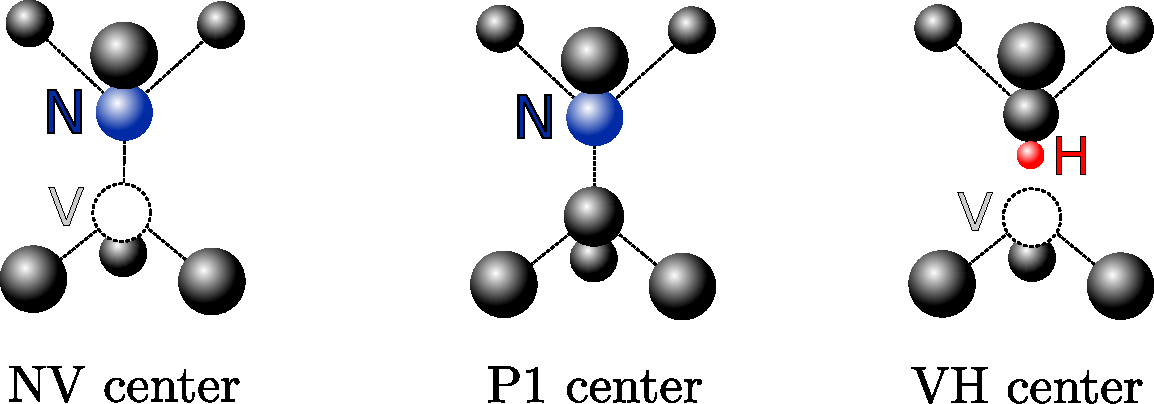
\includegraphics[width=\textwidth]{Figures/tronche_de_spin}
\caption{Crystalline structure of three spin defects: the NV center, the P1 enter (substituional Nitrogen) and the VH center.} 
\label{repr NV P1 VH}
\end{figure}

We refer by dark spins to paramagnetic impurities for which the spin degree of freedom is not accessible optically. At room temperature, only two defects in diamond do not have a dark spin: the NV center and the more recently found ST1 center \citep{lee2013readout, john2017bright}. Every other spin impurity identified so far is considered to be dark.

In this section we will present the most common dark spins encountered in diamond, which are simply the most common paramagnetic impurities aside from the NV center, and the relation between the diamond growth process and the presence of these impurities. We will also briefly present EPR spectroscopy which is the most common method to characterize these dark spins.

\subsection{P1 centers and $^{13}$C}
The most common spin defects in NV-rich diamond are the substitutional nitrogen centers N$^0_S$ known as the P1 centers (see Fig. \ref{repr NV P1 VH}), which have an electronic spin $1/2$ and a nuclear spin 1, and the $^{13}$C $1/2$ nuclear spin which represents 1.1\% of natural abundance carbon atoms, the remaining carbon atoms being almost exclusively the spinless $^{12}$C isotope. In NV-rich diamonds, these two impurities are the main causesof the NV center dephasing rates $\Gamma_2^*=1/T_2^*$ and $\Gamma_2=1/T_2$  \citep{barry2020sensitivity}. 

The dephasing rate caused by a given impurity is directly proportional to the average diagonal dipole-dipole matrix elements ($\Omega_{\rm shift}$ in (eq. \ref{eq. ff df})) between the two spin species \citep{taylor2008high, bauch2020decoherence}. Since the dipole-dipole interaction scales as $1/r^3$, and the distance $r$ between each spin scales as the inverse cubic root of the concentration,  it is expected that the dephasing rate associated with a particular impurity scales linearly with the concentration of the impurity: $\Gamma_2^*(\rm P1) \propto [P1]$. 

In the case of P1 centers, this was verified experimentally by looking at controlled sample with varying concentration of nitrogen \citep{bauch2020decoherence}. The authors of the study found a value of $\Gamma_2^*(\rm P1)= (2 \pi) 16\ \rm kHz/ppm$. For the samples studied in this manuscript [REF], the P1 concentration was 

$^{13}$C nuclei are typically much more abundant than P1 center ($\sim$ 10 000 ppm without istopic engineering) but being a nuclear spin, it has a gyromagnetic ratio $\approx 2.8\cdot 10^3$ times smaller than that of the P1. As a result, the contribution of a single $^{13}$C nucleus to the NV dephasing rate is $\sim 10^3$ times that of a single P1 center. It was found experimentally that the broadening caused by $^{13}$C is $\Gamma_2^*(^{13}\rm C ) \approx (2 \pi) 16\ \rm Hz/ppm$ \citep{van1997dependences, barry2020sensitivity}. In samples with natural isotopic abundance of carbon, the inhomogeneous dephasing rate due to the $^{13}$C nuclear spins has a value $\Gamma_2^*(^{13}\rm C ) \approx (2 \pi) 160\ \rm kHz$.

\subsection{Other spin defects, VH$^-$, War1}
\label{other defects}
Other spin defects are also commonly found in diamond containing NV centers, such as charged vacancy or vacancy clusters \citep{hounsome2006origin}, other nitrogen related defects \citep{newton2007epr}, transition metals \citep{isoya1990fourier}, and especially for CVD grown diamond, hydrogen related defects \citep{hartland2014study}, since the CVD plasma contains up to 95 \% hydrogen (see sec. \ref{fab HPHT}).

Of particular interest in this chapter are two defects: the VH$^-$ defect \citep{glover2003hydrogen, glover2004hydrogen} and the War1 defect \citep{cruddace2007magnetic}. 

The VH$^-$ defect, prior to our observations, had only been observed via electron paramagnetic resonance (EPR) in CVD grown diamond. It is formed by a vacancy with a hydrogen atom forming a bond with one of the four neighboring carbon atoms (see Fig. \ref{repr NV P1 VH}). To acquire its negtatively charged state, the VH center needs to capture an electron from a donor in the crystal, similarly to the NV center. 

This defect has a similar electronic structure as the NV$^-$ which results in an electronic spin-1 with a similar zero field splitting parameter (see Table \ref{table VH et War1}). Although the presence of hydrogen in this defect was confirmed by isotopic study, it has been debated whether this defect was VH$^-$ or V$_2$H$^-$ due to a conflict with \textit{ab initio} calculations \citep{shaw2005importance}. The defect is therefore sometimes referred to as V$_n$H$^-$. In this manuscript we will employ the original terminology: VH$^-$.

The War1 defect, named after the University of Warwick where it was first observed in a CVD diamond \citep{cruddace2007magnetic}, is another spin-1 defect whose chemical structure remains unknown. No hyperfine structure could be discerned in the relatively broad EPR line, and the use of deuterium instead of $^1$H did not change the shape of the line.

\subsection{EPR spectroscopy}
\begin{figure}[h!]
\centering
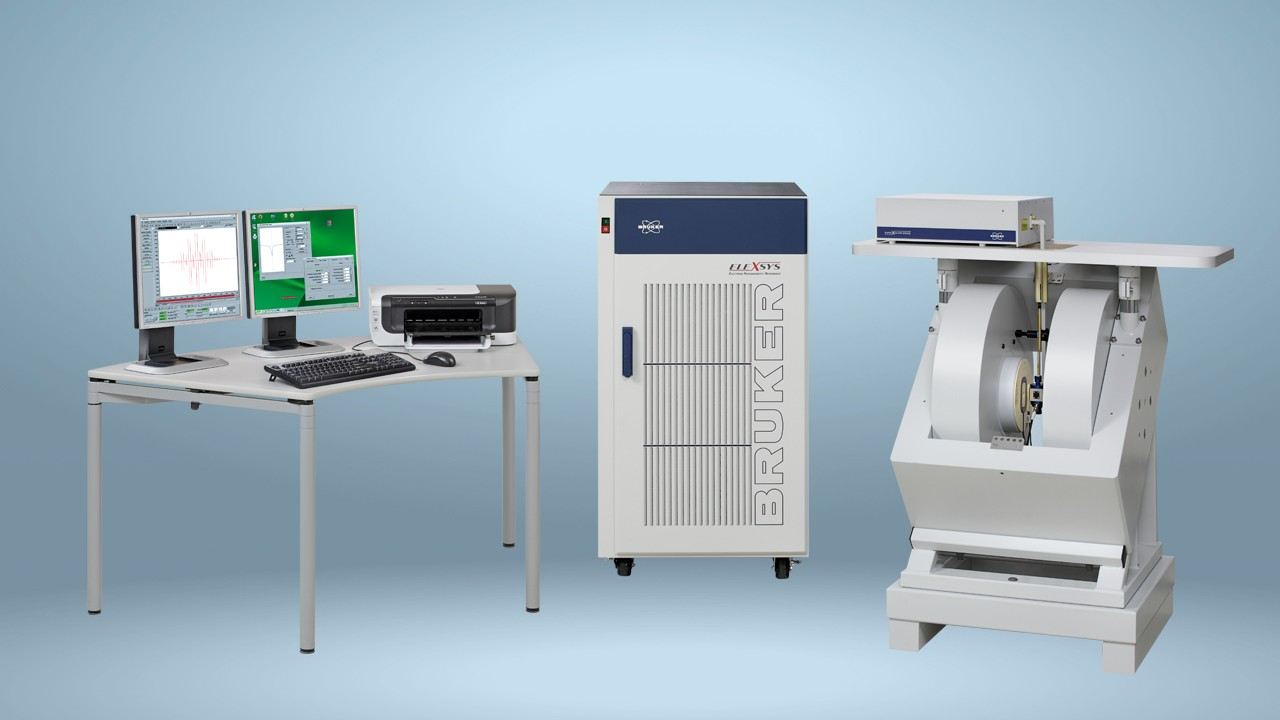
\includegraphics[width=.7\textwidth]{Figures/EPR_spectometer.jpg}
\caption{EPR specrometer. Credits: Bruker Corporation} 
\label{photo EPR}
\end{figure}

Electron paramagnetic resonance (EPR), the electronic equivalent to NMR, is the the most common way to detect electronic spins in solids and liquids. The principle of its detection is the absorption or reflection of a microwave field resonant with a spin transition.

EPR generally relies on the thermal polarization of the spins to observe an absorption. In order to increase the polarization, an important magnetic field is applied (typ. 0.35 T or 3500 G) and a microwave cavity (typ. 9500 MHz) is used to improve the coupling of the spins to the field.

The usual EPR apparatus, shown in Fig. \ref{photo EPR}, is a bulky and expensive lab equipment ($\gtrsim$ 1 M€). In contrast, optical detection such as ODMR is technically easier, less expensive, and allows better spatial resolution. 

ODMR can also be significantly more sensitive than EPR: single NV centers are routinely observed in ODMR while the the current EPR noise floor for electronic spins in diamond is typically of $\sim 10^{11}$ \citep{mitchell2013x}. This difference in sensitivity comes in part from the better spin polarization \footnote{At room temperature, the thermal polarization of a transition at 9500 MHz is $\sim 0.002$ while the NV center optical polarization can reach 0.8.}, and from the more efficient photon detection in the optical range than in the microwave range.

EPR however remains a far more versatile tool as only very few spin defects have the properties required for ODMR. The key idea of this chapter is to allow the optical detection of spin defects that do not show ODMR, by making them resonant with NV centers and observing NV cross-relaxation.

\section{NV center relaxometry}

Detection of dark spins via NV center cross-relaxation fall under the more general technique of NV relaxometry, which consists in measuring a modification of the NV center spin lifetime $T_1$. Relaxometry with NV centers has been used not only to measure cross-relaxation with dark spins \citep{van1989cross, holliday1989optical, epstein2005anisotropic, armstrong2010nv,   hall2016detection, wickenbrock2016microwave,  wood2016wide,  alfasi2019detection, lazda2021cross}, but also to probe the magnetic noise in the diamond environment coming from spins \citep{steinert2013magnetic}, ions\citep{tetienne2013spin}, free radicals \citep{nie2021quantum}or magnetic domains \citep{finco2021imaging}. 

The protocols used in NV relaxometry measure either directly the spin $T_1$, as detailed in sec. \ref{sec T1 NV}, or indirectly through the NV photoluminescence.

\subsection{PL and single$-\tau$ relaxometry protocols}
\begin{figure}[h]
\centering
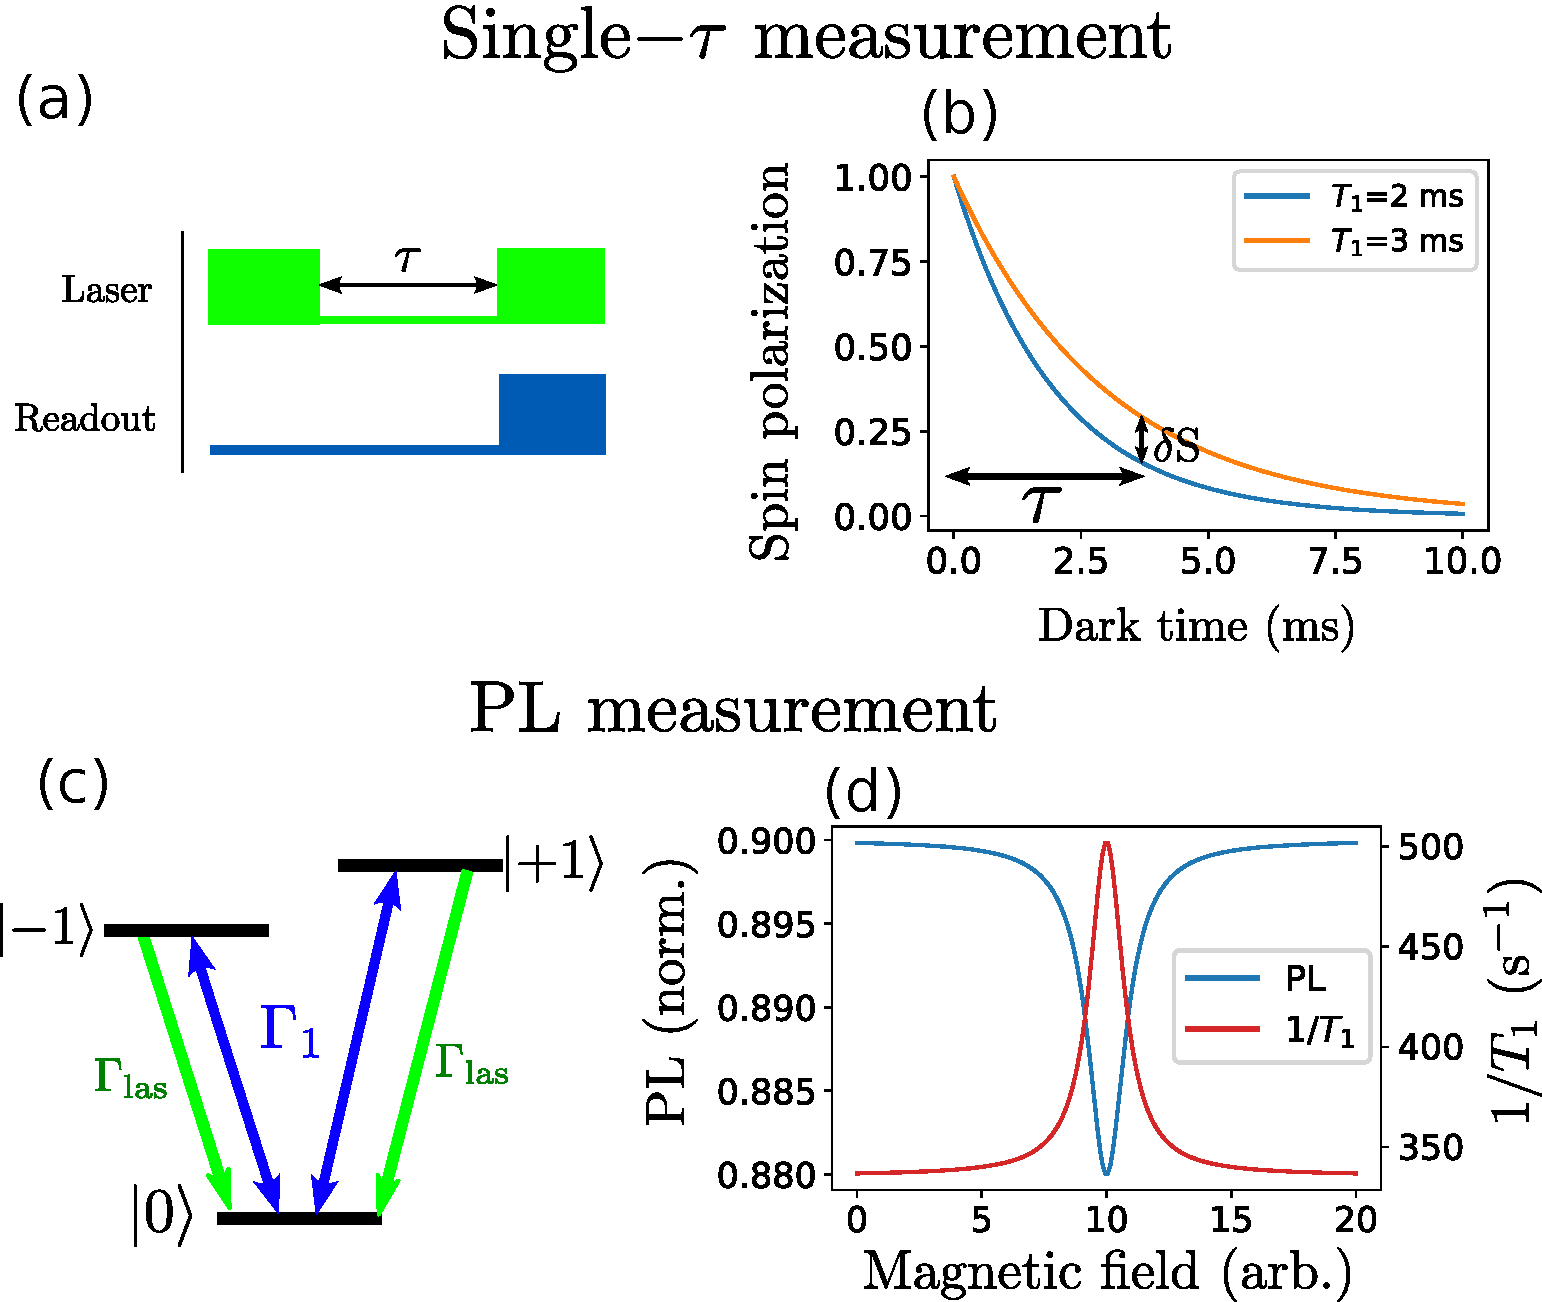
\includegraphics[width=0.9\textwidth]{Figures/relaxo_pulsed_continuous_2}
\caption{Representation of the two relaxometry protocol. (a) Simple $T_1$ measurement pulse sequence. (b) Simulation of two $T_1$ measurement with different $T_1$ values. $\tau$ represents the optimal dark time in order to maximize the signal $\delta S$ (c) Representation of the optical pumping (green arrows) and depolarization (blue arrows) of the NV center spin. (d) Simulation of the PL modification caused by a change in the spin $T_1$. The spin $T_1$ profile in term of the magnetic field was arbitrarily chosen.}
\label{T1 vs PL}
\end{figure}

The two most common protocols to perform NV relaxometry ar represented on Fig. \ref{T1 vs PL}. The first and most basic method simply consist in monitoring the PL of the NV centers : since the PL is proportional to the population in the $\ket{0}$ state, which itself results from an equilibrium between the polarization rate $\Gamma_{\rm las}$ and the spin decay rate $\Gamma_1=1/T_1$. A change in $\Gamma_1$ will therefore conduct to a new equilibrium with a different PL. 

The second method is a pulsed sequence referred as single$-\tau$ measurement, used for example in \citep{pelliccione2014two, schmid2015relaxometry, tetienne2016scanning}. It simply consists in a $T_1$ measurement sequence (as seen in chapter 1) where you first polarize the spins in the $\ket{0}$ state with a laser pulse and read out the spin state with a second laser pulse after a dark time $\tau$. In this case however, instead of scanning the time $\tau$, you fix its value to maximize the sensitivity in a change of $T_1$ (typically $\tau \approx T_1$). 

It is argued in \citep{finco2021imaging} that both methods result in similar signal to noise ratio: in the first case you need to adjust $\Gamma_{\rm las} \sim \Gamma_1$ to maximize the PL contrast, meaning that the laser power used is very far from the saturation limit (typically $\Gamma_1 \approx 10^3\ \rm s^{-1}$ and $\Gamma_{\rm sat} = 5\cdot10^6\ \rm s^{-1}$\citep{dreau2011avoiding}), while the second method needs to wait a time $\tau \sim T_1$ between each measurement, which result in a similar PL count and shot noise limit in both case.

On a technical level, the PL-based method is easier to implement since it does not require the use of a pulsed laser, and uses an overall smaller laser power, however it is more sensitive to drifts and changes in the optical setup. Most of the relaxometry measurement in this manuscript were performed using a PL-based detection.

\subsection{Comparison with DEER protocol}

\begin{figure}[h]
\centering
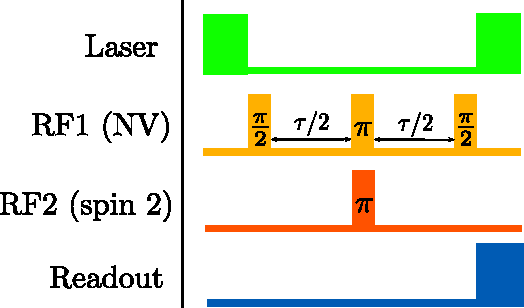
\includegraphics[width=0.5\textwidth]{Figures/DEER}
\caption{Pulse sequence of the DEER protocol}
\label{DEER}
\end{figure}

There can be several advantages to use relaxometry protocols, which measures a change in the NV $T_1$, over the more common magnetometry protocols that rely on a change in the NV $T_2$ or $T_2^*$: the first and most obvious one is that relaxometry does not need to use an external microwave field. This however comes at the cost of a greater precision needed on the external magnetic field. Relaxometry also allows AC-magnetic field sensing in the GHz regime \citep{wang2022picotesla, alsid2022solid}, while traditional microwave-based AC-megnetometry is limited to tens of MHz. Finally, relaxometry measurement can be more sensitive than the T2-based one in some instances \citep{steinert2013magnetic}, which comes from the fact that changes in NV $T_1$ times are easier to detect than changes in $T_2$ or $T_2^*$ since $T_1$ is much longer than $T_2$ or $T_2^*$.

Outside of cross-relaxations, another protocol exists to address dark spin resonance with NV centers, based on a modification of the NV $T_2$ time \citep{serbyn2014interferometric}. This protocol called double electron-electron resonance (DEER) is depicted on Fig. \ref{DEER}. The pulse sequence consist in a spin-echo sequence on the NV center, as described in chapter 1, with a simultaneous $\pi-$pulse on the probed dark spins during the rephasing pulse on the NV centers. This additional pulse means that the static (or slowly variable) contribution of the probed spins to the $T_2^*$ of the NV center wont be rephased. The newly measured $T_2$ time should therefore be slightly shorter:

\begin{equation}
\frac{1}{T_2^{\rm DEER}}=\frac{1}{T_2^{\rm echo}} + \delta \Gamma_2^*,
\end{equation}

where $\delta \Gamma_2^*$ is the contribution of the dark spin to the $T_2^*$ of the NV center.

By scanning the frequency of the second microwave (RF2) and monitoring the $T_2$ time of the NV centers, one can therefore find dark spin resonance without having to bring them to resonance with NV centers, which can be useful when the dark spin resonance is very far detuned from the NV one.

While both cross-relaxation and DEER measure the dipole-dipole coupling of dark spins to an NV center, there are several differences between the two protocols:

Frist, the two protocols do not measure the same elements of the dipole-dipole Hamiltonian: CR measures the off-diagonal elements $\Omega_{\rm CR}=\mel{i,j}{\mathcal{H}_{\rm dd}}{j,i}/\hbar$ which are responsible for the flip-flops or double flips, while DEER measures the diagonal elements $\Omega_{\rm DEER}=\mel{i,j}{\mathcal{H}_{\rm dd}}{i,j}/\hbar$ which are responsible for the pure dephasing. These terms however are on average of the same amplitude, and when averaging over an ensemble we can consider $\Omega_{\rm CR} \sim \Omega_{\rm DEER}$

Second and more importantly, the scaling is not the same in both cases : CR measures a change in the NV decay rate $\Gamma_1=1/T_1$ which is proportional to $\Omega_{\rm CR}^2$, as given by eq. \ref{delta gamma 1}, while DEER measures a change in $\Gamma_2=1/T_2$ which is proportional to $\Omega_{\rm DEER}$, as given by eq. \ref{Gamma2 P1}. This means that the signal of CR scales quadratically with the impurity concentration, while the DEER signal scales linearly with it. CR is therefore more suited to probe concentrated impurities, when the average distance between the NV and the probed spin is small.

\section{Choice of the magnetic field orientation}

Since relaxometry does not rely on a microwave field, the only parameter left to tune is the external magnetic field, which is often scanned with an electromagnet. Due to the strong NV anisotropy however, the direction along which $\mathbf{B}$ is scanned plays a crucial role in the ability to detect dark spins.

\subsection{The [100] and [111] magnetic field orientations}
\label{sec simu}

\begin{figure}[h]
\centering
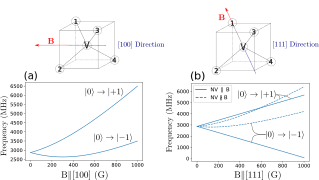
\includegraphics[width=0.9\textwidth]{Figures/121_vs_22_NV}
\caption{Simulated transition frequencies of the $\ket{0} \to {-1}$ and $\ket{0} \to {+1}$ transitions for the 4 classes of NV centers as a function of the magnetic field. a) When the magnetic field is along the diamond [100] crystalline axis, b) along the [111] axis. A representation of the 4 classes of NV centers, labeled 1 to 4, and the orientation of the magnetic field in both cases is put on top}
\label{121 vs 22 NV}
\end{figure}

Fig. \ref{121 vs 22 NV} shows the two main choices of scanning orientation : either $\mathbf{B} \parallel [100]$ or 
$\mathbf{B} \parallel [111]$ where [100] and [111] refer to the diamond crystalline axes as defined in chapter 1. When $\mathbf{B} \parallel [100]$, all four classes (the different possible NV orientations represented at the top of the figure) are equivalent, whereas for $\mathbf{B} \parallel [111]$, one class is perfectly aligned with the magnetic field while the three others are equivalently unaligned. 

These changes in the field orientation result in massive changes in the NV behavior, manly due to the transverse magnetic field: Fig. \ref{121 vs 22 NV}-a) shows the transition frequency between the $\ket{0}$ and $\ket{\pm 1}$ states of the ground state spin Hamiltonian (REF chapter 1) - or to be more precise the transitions between the ground state of the spin Hamiltonian and the two excited states - for any of the four classes of NV centers when $\mathbf{B} \parallel [100]$. Notably, there is no transitions frequencies below 2500 MHz. 

On the other hand, Fig. \ref{121 vs 22 NV}-b) shows the transition frequencies when $\mathbf{B} \parallel [111]$, for both the class aligned and the three class misaligned. The three classes behave similarly than the four classes in the $[100]$ case, but the one class aligned with the magnetic field can get its $\ket{0}\to\ket{-1}$ transition arbitrarily small, as long as the magnetic field is perfectly aligned with the NV axis.

\subsection{CR condition between NV$^-$ and P1}

\begin{figure}[h]
\centering
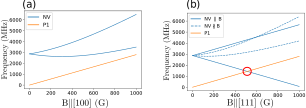
\includegraphics[width=0.9\textwidth]{Figures/121_vs_22_P1}
\caption{Simulation of the transition frequencies of NV$^-$ centers and P1 centers (without the hyperfine interactions) for a magnetic field a) along the [100] axis and b) along the [111] axis}
\label{121 vs 22 P1}
\end{figure}

P1 centers, the most abundant electronic spin in the diamonds commonly used, have a $1/2$ electronic spin. They do have a small magnetic field anisotropy coming from the hyper-fine coupling to the nitrogen nucleus ($\sim 100\ \rm MHz$), but this dependency on the field orientation is small compared to the NV center's zero field splitting $D=2870\ \rm MHz$. We can therefore, to the first order, neglect the hyper-fine coupling and consider P1 centers as ideal, isotropic, spin $1/2$.

Fig. \ref{121 vs 22 P1} shows the transition frequencies for the NV center and such a spin $1/2$, as a function of a magnetic field parallel to [100] or [111]. When $\mathbf{B} \parallel [100]$, there will never be a co-resonance between the NV and P1 transitions, meaning that no NV-P1 cross-relaxation can be observed when B is scanned in this direction. When $\mathbf{B} \parallel [111]$ however, the P1 $\ket{-1/2} \to \ket{+1/2}$ transition matches in energy the $\ket{0}\to\ket{-1}$ NV transition for B=512 G. This means that when B reaches $\approx 512\ \rm G$, some of the polarization of the NV centers will be transferred to the P1 centers, which will result in a drop in the NV PL. 

\subsection{CR condition between NV$^-$ and VH$^-$}

\begin{figure}[h]
\centering
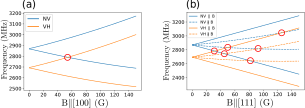
\includegraphics[width=0.9\textwidth]{Figures/121_vs_22_VH}
\caption{Simulation of the transition frequencies of NV$^-$ centers and VH$^-$ centers for a magnetic field a) along the [100] axis and b) along the [111] axis}
\label{121 vs 22 VH}
\end{figure}

VH$^-$, a much less abundant electronic spin than P1 center, has an electronic spin 1, with a spin Hamiltoninan very similar to that of the NV center. In particular it has the same symmetries being also a $C_{3v}$ defect, with a slightly smaller ZFS at $D_{VH} \approx 2700\ \rm MHz$ compared to $D_{NV}=2870\ \rm MHz$. 

Fig. \ref{121 vs 22 VH} shows the transition frequencies for the NV$^-$ and VH$^-$ ground state spin. Contrary to the P1 case, there is a co-resonance when $\mathbf{B} \parallel [100]$ for $B\approx 55\ \rm G$. When $\mathbf{B} \parallel [111]$, there are 6 co-resonance conditions between 30 and 130 G. A scan along the [111] in this case means that the peak signal will be $\sim 6$ times weaker than in the [100] case, and spread over multiple lines which might overlap between themselves or with other existing PL features.

The War1 spin mentioned previously is also an electronic spin 1 with (pseudo)-$C_{3v}$ symmetry and $D_{War1} \approx 2470\ \rm MHz$. This result in a similar behavior than VH$^-$ when it comes to the CR condition with NV centers.

\subsection{CR condition between NV$^-$ and and $^{13}$C-NV$^-$}

\begin{figure}[h]
\centering
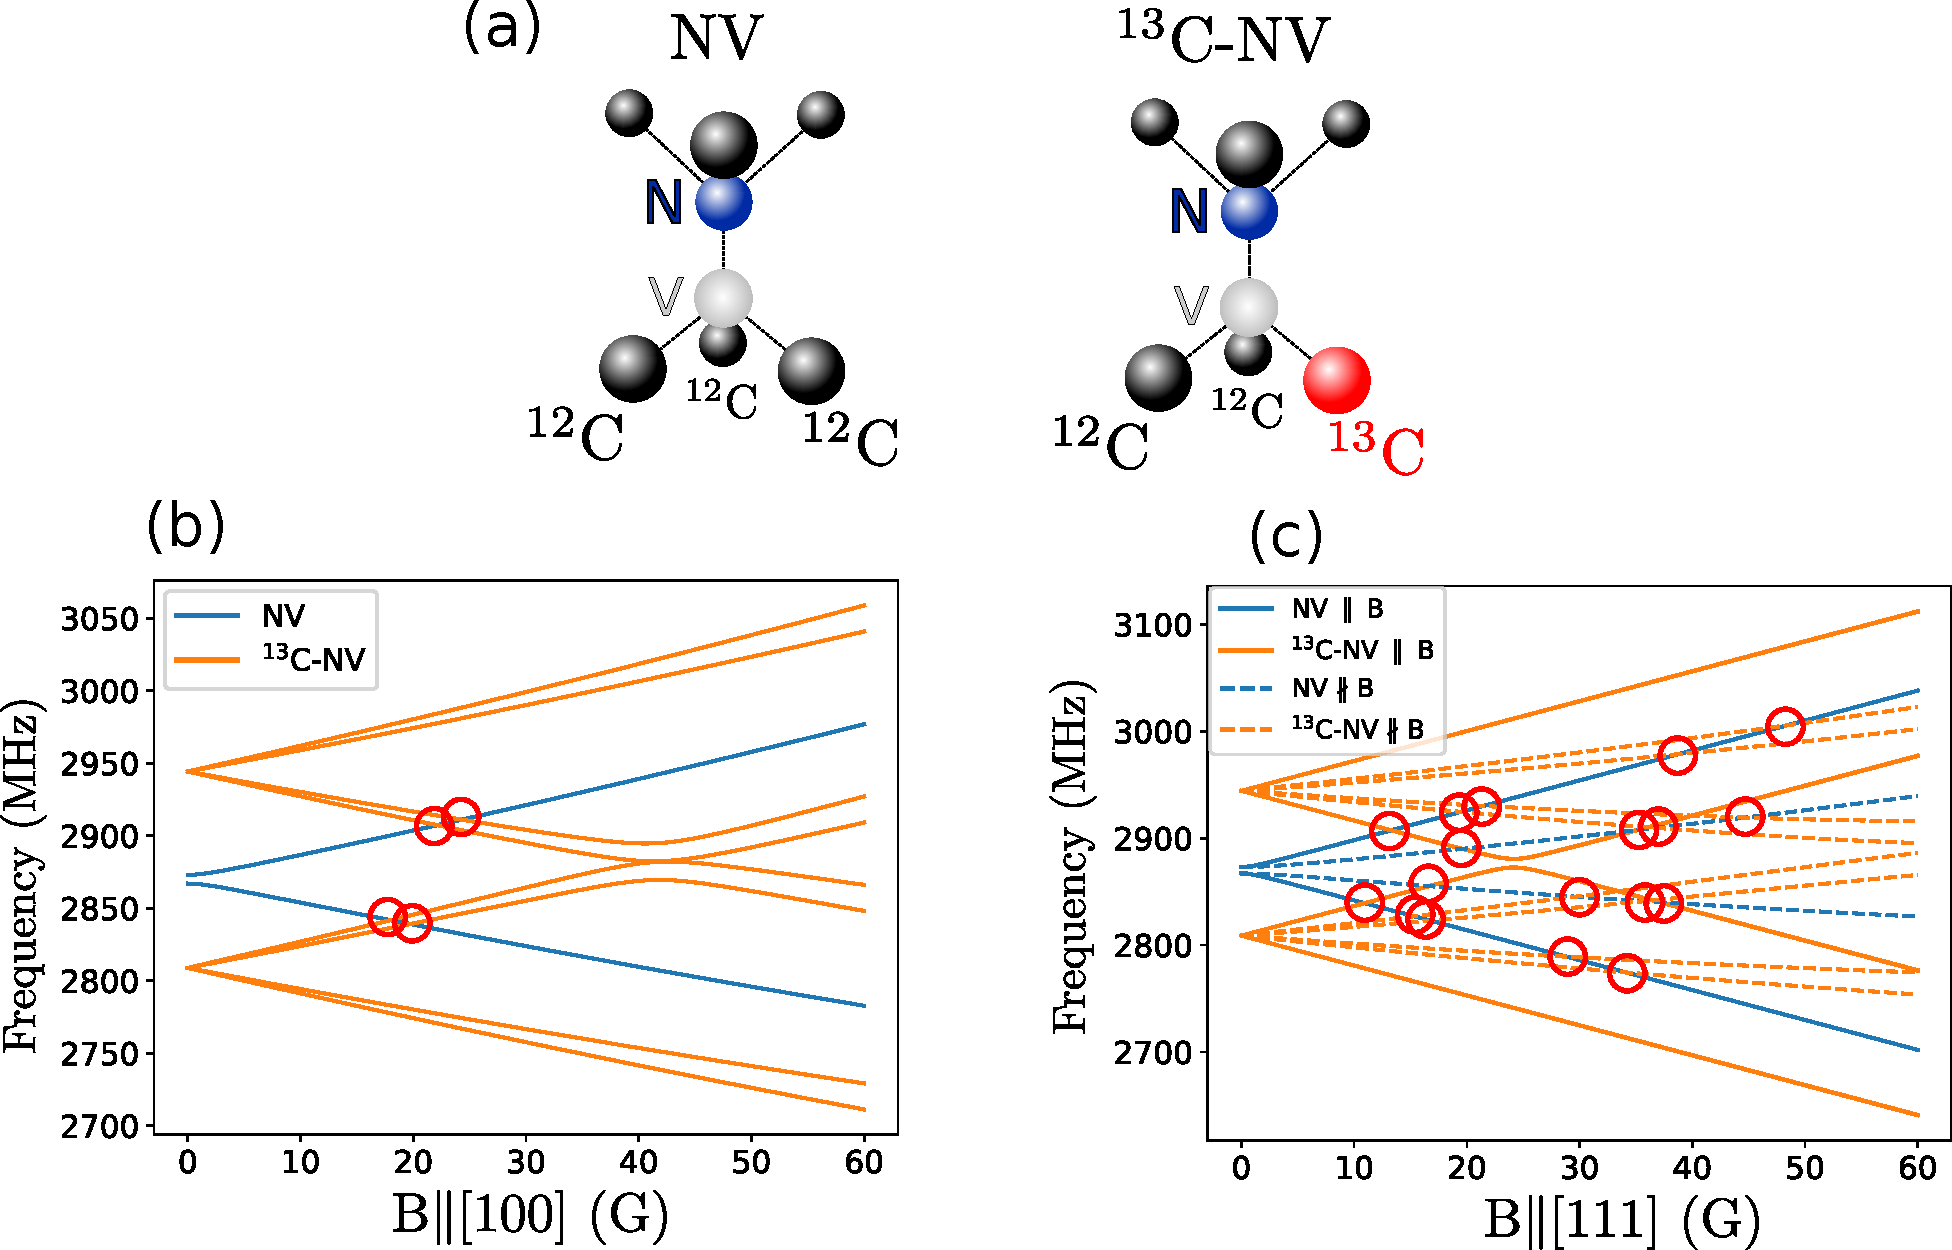
\includegraphics[width=1\textwidth]{Figures/121_vs_22_13CNV}
\caption{a) Representation of the $^{13}$C-NV complex (right) compared to a ``normal" NV center (left) b) and c) simulation of the transition frequencies of NV$^-$ centers and $^{13}$C-NV$^-$ complex for a magnetic field b) along the [100] axis and c) along the [111] axis}
\label{121 vs 22 13C-NV}
\end{figure}

I refer by $^{13}$C-NV$^-$ to a complex formed by an NV center where one of the three carbon atoms neighboring the vacancy is a $^{13}$C isotope. Such a complex is illustrated in Fig. \ref{121 vs 22 13C-NV}-a).

The $^{13}$C-NV$^-$ complex still behaves as a ``normal" NV center, except that its transition lines are shifted by the hyper-fin coupling. In particular its electronic spin is still polarized in the $\ket{0}$ state and the $\ket{0}$ state is still brighter than the $\ket{\pm 1}$ states. This is confirmed by the presence of sideband in ODMR spectra around the main NV lines \citep{simanovskaia2013sidebands}.

Since both NV$^-$ and $^{13}$C-NV$^-$ are \textit{a priori} equally polarized, then following the argument in \ref{Sec_CR} there should be no CR between the two spin families. The reason why those transitions are still in some case visible, as will be shown below, and why in fact any NV-NV co-resonance gives a visible CR signal will be the object of the next chapter.

The transitions of the $^{13}$C-NV$^-$ complex are given by diagonalizing the full spin Hamiltonian:
\begin{equation*}
\mathcal{H}=\mathcal{H}_{NV}+\mathcal{H}_{^{13}C}+\mathcal{H}_{HF},
\end{equation*}
where $\mathcal{H}_{NV}$ is the NV$^-$ spin Hamiltonian,
$\mathcal{H}_{^{13}C}$ is the $^{13}$C nuclear spin Hamiltonian for a $1/2$ spin : $\mathcal{H}_{^{13}C}=\gamma_{n} B I_z$ where $\gamma_{n}=$10.7 MHz/T is the $^{13}$C gyromagnetic ratio, and $\mathcal{H}_{HF}$ is the hyper-fine interaction Hamiltonian: $$\mathcal{H}_{HF}= \hat{\mathbf{S}}_{NV} \cdot \mathcal{A} \cdot \hat{\mathbf{I}}_C.$$

When the $^{13}$C is the direct neighbor of the vacancy as represented in Fig. \ref{121 vs 22 13C-NV}-a) - this is also referred as a first-shell $^{13}$C - the hyper-fine tensor $\mathcal{A}$ can be written \citep{simanovskaia2013sidebands}:
$$ \mathcal{A} = \begin{pmatrix}
\mathcal{A}_{xx} & 0 & \mathcal{A}_{xz} \\ 0 & \mathcal{A}_{yy} & 0 \\ \mathcal{A}_{zx} & 0 & \mathcal{A}_{zz}
\end{pmatrix},$$
where $\mathcal{A}_{xx}=190$ MHz, $\mathcal{A}_{yy}=120$ MHz, $\mathcal{A}_{zz}=129$ MHz, and  $\mathcal{A}_{xz}=\mathcal{A}_{zx}=-25.0$ MHz. 

Fig. \ref{121 vs 22 13C-NV}-b) and c) show the simulated transition frequencies for a $^{13}$C-NV$^-$ complex when B is scanned along the [100] or [111] axis, as well as the ``normal" NV transitions and the co-resonance between those two. When $\mathbf{B} \parallel [100]$, there are 4 co-resonances between 18 and 25 G. When $\mathbf{B} \parallel [100]$ there are 18 of them between 10 and 60 G. This abundance of transitions for low ($<100\ \rm G$) magnetic field makes analyzing experimental data quickly intractable in the second case.

\subsection{CR contrast and transverse magnetic field}
\label{CR contrast}

\begin{figure}[h]
\centering
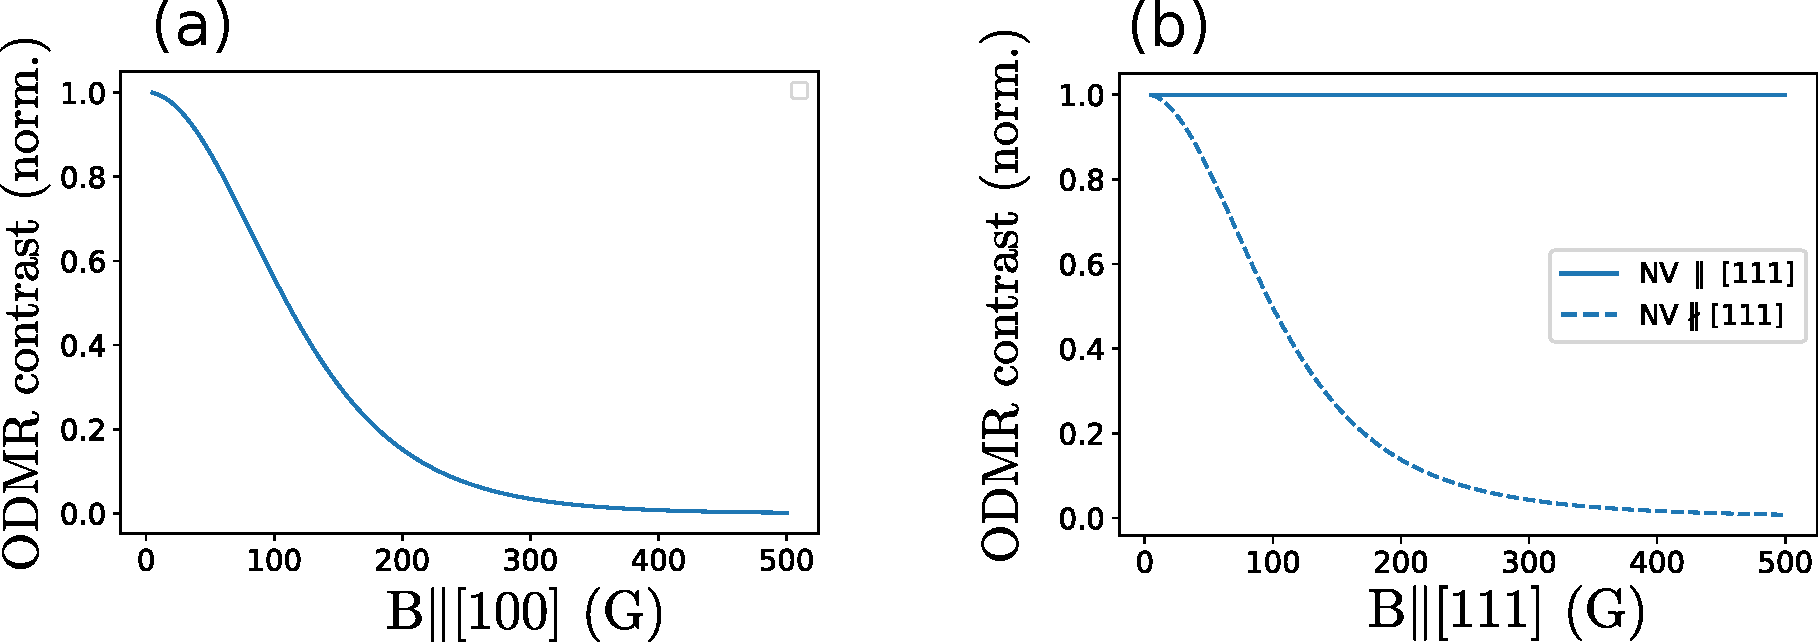
\includegraphics[width=0.9\textwidth]{Figures/contrast_OMDR_111_Vs_100}
\caption{Simulated ODMR contrast on all four classes of NV centers with a magnetic field a) along the [100] axis and b) along the [111] axis}
\label{121 vs 22 contrast}
\end{figure}

In order to optically detect CR between an NV center and a dark spin, two conditions must be met: the NV center must be polarized in order to have a population transfer between the NV and the dark spin, and there must be a difference in brightness between the two NV levels involved in order to have an optical signature of the CR.

These two conditions are in fact the same needed to observe an ODMR spectrum (REF chapter 1), and while the NV centers verifies both criteria in presence of a purely longitudinal magnetic field, this is not always the case anymore in presence of a transverse magnetic field (REF chapter 1).

Fig. \ref{121 vs 22 contrast} shows the simulated relative contrast of an ODMR spectrum, as computed from \citep{tetienne2012magnetic}, for a magnetic field aligned along [100] or [111]. When the NV center is aligned with the magnetic field, the constrats remains equals to 1 regardless of the magnetic field because there is no transverse field. When the NV is not aligned however, either in the [111] or [100] case, the ODMR contrast quickly drops down for B$>100\ \rm G$.

This tells us that we should not expect to observe a CR signal for B greater than a few hundreds G when B is scanned along the [100] axis. We could however observe CR for arbitrarily large magnetic field when scanned along the [111] axis, as long as the field is properly aligned with the NV axis.

\section{Dark spin spectroscopy with NV centers}

\subsection{Detection of P1 centers}

\begin{figure}[h]
\centering
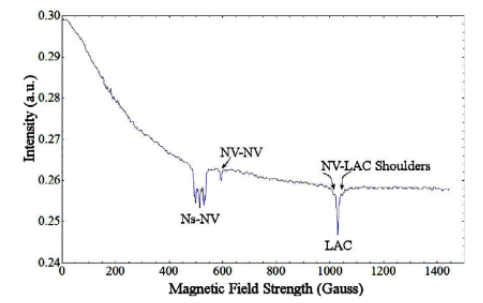
\includegraphics[width=0.7\textwidth]{Figures/NV_P1_libreAcces}
\caption{Change in the PL of an ensemble of NV centers as a magnetic field is scanned along the [111] crystalline axis. Taken from \citep{armstrong2010nv}}
\label{CR P1 exp}
\end{figure}

Previously to our work, several studies \citep{van1989cross, holliday1989optical, epstein2005anisotropic, armstrong2010nv,   hall2016detection, wickenbrock2016microwave,  wood2016wide,  alfasi2019detection, lazda2021cross} had been done on the detection of dark spins through CR with NV centers, and to our knowledge, all this studies where done on the detection of P1 centers. Following the discussion in the last section, these studies were therefore all done with $\mathbf{B} \parallel [111]$.

An example of one of this study (\citep{armstrong2010nv}) is shown in Fig. \ref{CR P1 exp}. It shows the evolution of the NV PL with respect to a magnetic field scanned along the [111] crystalline axis. There are several information to gather from this graph:

First, there is the slowly decaying PL envelope, which stabilizes to a plateau for $B\sim 1000\ \rm G$. This change in PL is caused by the transverse magnetic field acting on the three NV classes that are not aligned with the magnetic field. For $B \gtrsim 1000\ \rm G$, these three classes are fully depolarized which explains the plateau observed.

Second, there are the three salient features denoted Ns-NV, NV-NV and NV-LAC. All these features come from cross-relaxations or level anti-crossing (LAC) from the NV class aligned with the magnetic field.

The first feature (Ns-NV) for $B\approx 512 \ \rm G$ is the signature of the CR between NV and P1 centers. Its relatively complicated shape comes from the hyper-fine coupling between the P1 electronic spin and the $^{14}$N nucleus \citep{lazda2021cross}. Excited state level anti-crossing (ESLAC) also occurs in this region, but its optical signature, if it exists, is expected to be much weaker than the NV-P1 CR \citep{zheng2017level}.

The second feature (NV-NV) for $B\approx 590 \ \rm G$ comes from the cross relaxation between NV centers aligned with the magnetic field and NV centers misaligned with the field (the co-resonance can be observed in Fig. \ref{121 vs 22 NV}-b)). This phenomenon will be further discussed in the next chapter.

Finally the third feature (LAC) for $B\approx 1024 \ \rm G$ correspond to the level anti-crossing between the $\ket{0}$ and $\ket{-1}$ states of the NV center aligned with B. When the two levels get close enough in energy, the Hamiltonian off-diagonal terms (coming from strain local electric field or residual transverse magnetic field) will mix the $\ket{0}$ and $\ket{-1}$ states and prevent an efficient polarization by the green laser. This result in a sharp drop in the PL that can be exploited to perform microwave-less magnetometry with NV centers \citep{wickenbrock2016microwave, zheng2017level, zheng2020microwave}.

\subsection{Detection of VH$^-$, War1 and $^{13}$C-NV$^-$}

\begin{figure}[h]
\centering
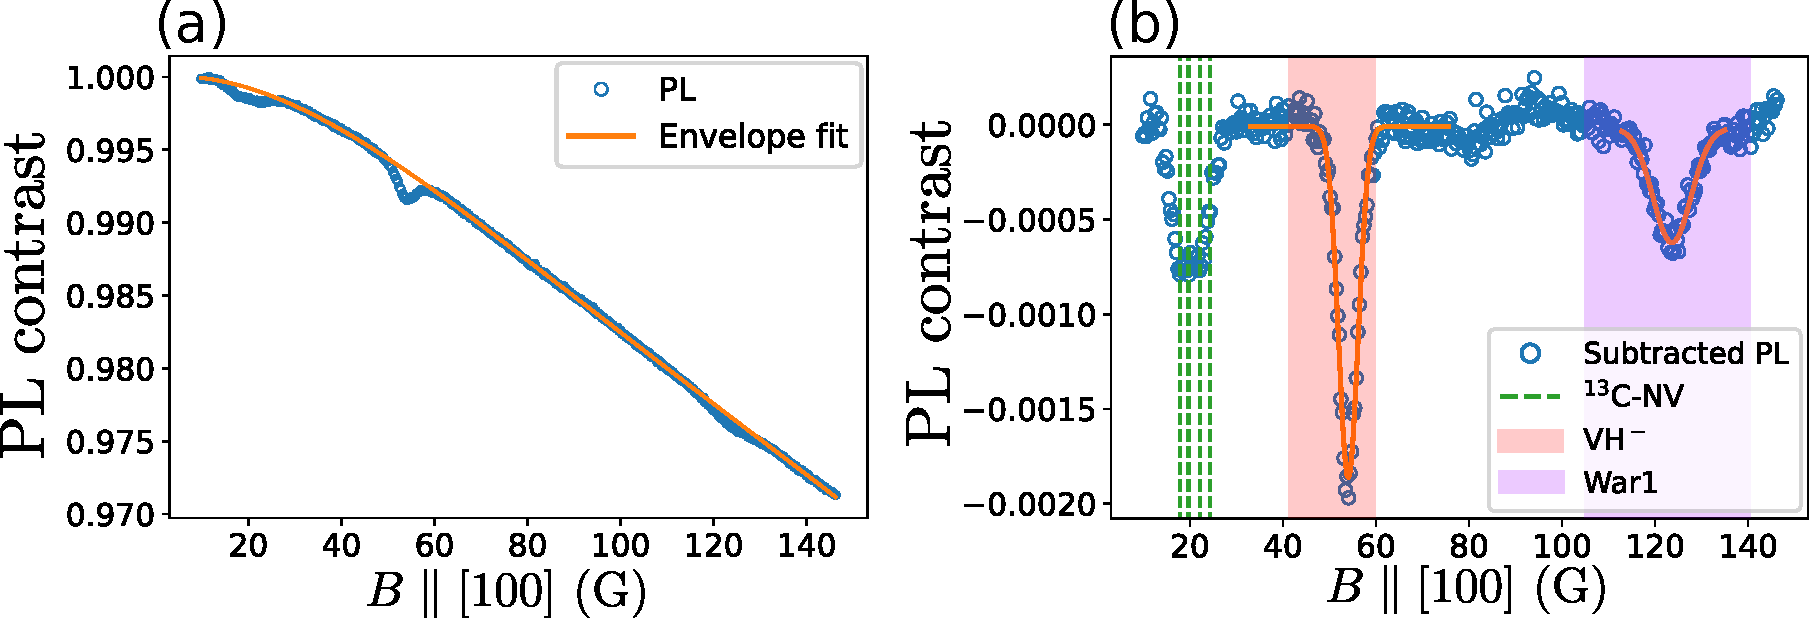
\includegraphics[width=\textwidth]{Figures/fig_VH_et_co}
\caption{a) Change in PL (normalized) of the ensemble of NV centers in sample CVD-pink as a magnetic field is scanned along the [100] axis. The orange line is a fit to the slowly decreasing envelope b) Subtraction of the PL signal by the envelope fit as a function of the magnetic field. The green lines and red and purple regions correspond to the predicted CR regions, as detailed in main text}
\label{CR VH exp}
\end{figure}

Our work \citep{pellet2021optical} focuses on the optical detection of VH$^-$, War1 and $^{13}$C-NV$^-$ through NV CR. This study was the first to detect VH$^-$ and War1 defects optically and the first CR experiment on a CVD diamond. It was also the first,to our knowledge, to use a [100] aligned magnetic field.

The diamond used for this study is the sample CVD-pink [REF appendix] whose fabrication was detailed in \citep{tallaire2020high}. It is a CVD diamond containing $[\rm NV ]\approx 4\ \rm ppm$ for $[\rm N ]\approx26\ \rm ppm$, and a natural abundance (1.1\%) of  $^{13}$C. Being a CVD diamond it is also likely to incorporate hydrogen defects, as discussed in \ref{other defects}.

Fig. \ref{CR VH exp}-a) shows the change in PL with respect to a magnetic field scanned along the diamond [100] axis. Similarly to fig. \ref{CR P1 exp}, we can see a slowly decaying envelope of the PL due to the transverse magnetic field (we don't see the plateau here since the magnetic field stops at 150 G). We can also see three deviations to the smooth decreasing curve at $\sim$ 20 G, 55 G and 120 G.

In order to better discern the three features, we fitted the envelope by using a polynomial fit of order 4 on the smooth part of the data. We previously tried to use a fit based on the expected PL rate of the NV centers, by using the model in \citep{tetienne2012magnetic}, but the results were not satisfying.

Fig. \ref{CR VH exp}-b) shows the subtraction of the PL data by the envelope fit. We can clearly see three dips in PL around the values 20 G, 56 G and 122 G. We then computed the expected value of the magnetic field for the expected CR line thanks to the simulations shown in sec. \ref{sec simu}. For the VH$^-$ and War1 lines, we took the ZFS $D$ values from \citep{cruddace2007magnetic} and included the error bars. For the $^{13}$C-NV$^-$ lines, the error bars given in \citep{simanovskaia2013sidebands} are much smaller and we only plotted the expected value. We can see that the dips in PL match relatively well the predicted CR lines of $^{13}$C-NV$^-$, VH$^-$ and War1 respectively.

The experimental setup used to obtain this data is the standard confocal microscopy setup shown in appendix REF. The magnetic field here is generated with an electromagnet (EM), aligned along the [100] diamond axis with a precision $<1^\circ$. 

The data shown here was acquired over 24 h. It should be noted however that a single-photon counting APD was used here, which considerably worsens the sensitivity of the measurement as discussed in [REF]. Using a photodiode and modulation of the magnetic field, we estimate that we could get similar signal to noise ratio within a few minutes.

To calibrate the magnetic field, we added a microwave field at a  fixed frequency $\nu > 2870\ \rm MHz$, and measured the EM voltage at which the PL dropped due to the $\ket{+1}$ state of the NV centers becoming resonant with the microwave tone. We could then use the values in Fig. \ref{121 vs 22 NV} to find the corresponding magnetic field. We varied the frequency in the range  $[2870,3150]\ \rm MHz$ by step of 2 MHz to get a calibration of the magnetic field in the $[0,150]\ \rm G$ region. Considering the uncertainty in the field angle, the NV ZFS $D$ value and the width of the PL drop, we estimate the final precision of the calibration to be within $\pm 1\ \rm G$.

\section{Attribution of the $^{13}$C-NV$^-$, VH$^-$ and War1 lines}

\subsection{The VH$^-$ and War1 lines}
\begin{table}[htbp]
\centering
\caption{\bf Zero-field splitting parameter $D$ for NV$^-$, VH$^-$ and War1}
\begin{tabular}{ccc}
\hline
$D_z$ estimation (MHz) & Cruddace's work\citep{cruddace2007magnetic} & Our work \\
\hline
NV$^-$ & 2872(7) & * \\
VH$^-$ & 2706(30) & 2694(5)  \\
WAR1 & 2466(60) & 2470(10) \\
\hline
\end{tabular}
  \label{table VH et War1}
\end{table}

The attribution of the PL dips at 56 and 122 G in Fig. \ref{CR VH exp} to CR between NV and respectively VH$^-$ and War1 comes from two main observations: the closeness in the ZFS values, and the CVD nature of the sample.

Table \ref{table VH et War1} shows the value and precision of the $D$ factor when measured through EPR \citep{cruddace2007magnetic}, and when computed from the data in Fig. \ref{CR VH exp}. In order to get to the $D$ value of VH$^-$ and War1, we had to assume that the spin structure was that of a spin 1 similar to the NV center, with a g-factor close to 2. Both of this assumptions are confirmed by the EPR measurements. We do find that that both $D$ measurement concord within their respective error bars.

The second reason comes from the nature of the sample used. We tried similar PL scans along the [100] axis on many samples with dense ensemble of NV centers. We found that the dip at 55 G was present on all CVD samples ($\sim$ 5 samples) used, and none of the HPHT samples ($\sim$ 20 samples). The same is true of the 122 G line, except that it did appear on some HPHT samples, as will be discussed below. We know that the VH$^-$ defect is much more likely to appear in a CVD sample due to the large quantity of hydrogen used in the process, and while we don't know the chemical nature of the War1 defect, the only time it was observed through EPR was on a CVD diamond.

Finally, the apparent larger linewidth of the War1 line compared to the VH$^-$ one is also corroborated by the EPR measurements.

For all of this reasons we attribute the 55 and 122 G dip to CR with VH$^-$ and War1 respectively, with a slightly stronger confidence for the VH$^-$ since more is known about it.

\subsection{The $^{13}$C-NV$^-$ lines}

\begin{figure}[h]
\centering
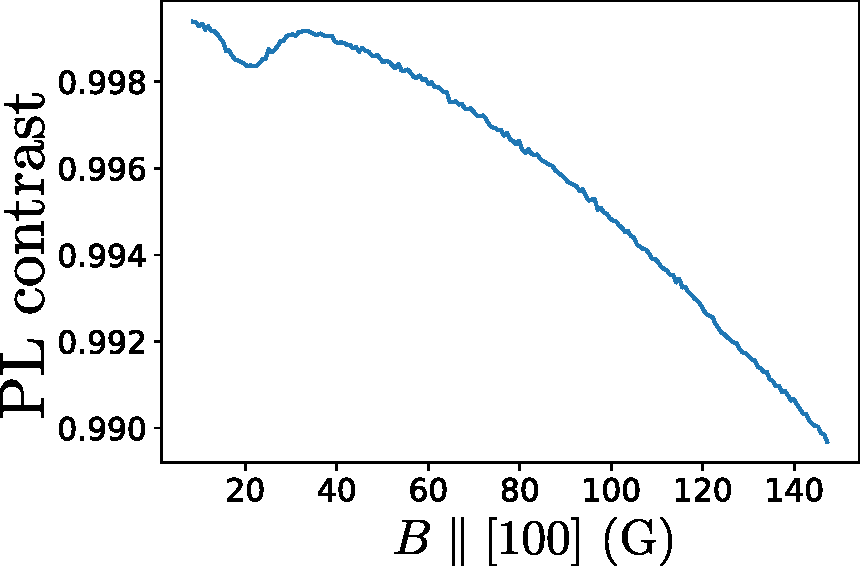
\includegraphics[width=.6\textwidth]{Figures/scan_100_Sumi4}
\caption{Change in PL as a function of a magnetic field scanned along the [100] axis for sample SUMI-4}
\label{scan sumi 4}
\end{figure}

The attribution of the $\sim 20\ \rm G$ dip to CR with $^{13}$C-NV$^-$ also come from two observations. First, the lines are present on every single sample with dense ensemble ($\gtrapprox 1$ ppm), regardless of the fabrication process. Fig. \ref{scan sumi 4} for example shows a PL scan along the [100] axis for sample Sumi-4, an HPHT sample with [NV]$\approx 5\ \rm ppm$ and natural abundance of $^{13}$C. I could unfortunately not try a sample isotopically enriched in $^{12}$C since those samples are generally reserved to low-nitrogen concentration ($< 10\ \rm ppm$), which does not yield enough NV centers to perform CR spectroscopy. 

The second reason is the shape of the PL dip. The two other dips seem be formed of a single line and are reasonably well fitted with Gaussian curves. The 20 G dip however has a flat bottom which would indicate the presence of several overlapping lines, and Fig. \ref{121 vs 22 13C-NV} indeed predicts that there would be 4 CR lines between 18 and 25 G.

For this two reasons, we attribute the 20 G line to CR between $^{13}$C-NV$^-$ and ``normal" NV centers.

\section{Quantitative estimates of the NV-Dark spins CR}

We can extract some quantitative information about the dark spins by exploiting the CR spectrum shown in Fig. \ref{CR VH exp}.

\subsection{Dark spin Hamiltonian parameters}

First, as discussed in the last section, we can estimate the dark spin ZFS $D$ value with greater precision than EPR. While it would be in theory possible to measure other properties of the dark spins Hamiltonian - such as the $g$-factor - by changing the angle of the magnetic field, this would here quickly become intractable due to the increase in co-resonance conditions and the relative closeness of each of these transitions. DEER might prove more useful in this regard as only one class of NV centers at a time is probed.

\subsection{Dark spin linewidth}

The second quantitative estimate we can make is of the dark spin inhomogeneous broadening $T_2^*$: if we assume the change in PL to be proportional to the change in the NV lifetime $T_1$, which is true for small enough changes, then the linewidth of the PL dips in Fig. \ref{CR VH exp} is the convolution of the NV and dark spin spectrum. By deconvoluting the data with the NV spectrum, known for example from ODMR, we can then recover the dark spin spectral response as was done in \citep{hall2016detection}. 

This procedure will be discussed in more details in the next chapter. We find here that the linewidth of VH$^-$ and War1 are respectively [REF] and [REF] MHz.

\subsection{Dark spin concentration}

Finally, the third tentative estimate we can make is that of the dark spins concentration. We can indeed calibrate the measurement by using the $^{13}$C-NV$^-$ line, of which we know the concentration in natural abundance diamond: [$^{13}$C-NV$^-$] $\approx$ 3.3 \% [NV]. We can then, knowing the NV concentration, try to estimate the concentration of the dark spins. There are several caveats though:

\begin{itemize}
\item Since the change in $T_1$ is proportional to the $T_2^*$ of the probed spins (eq. \ref{delta gamma 1}), we should compensate that by integrating over the entire feature, instead of simply looking at the maximum of the line.
\item We have to take into account the loss of contrast of the NV centers as the transverse magnetic field grows, as explained in sec. \ref{CR contrast}.
\item The $^{13}$C-NV$^-$ are not ``dark spins", and its CR feature cannot be \textit{a priori} compared to the one from VH$^-$ and War1. We will see however in the next chapter that we can consider a fraction of the NV centers as dark spins, and that this fraction can be estimated. \citep{choi2017depolarization} found a ratio of $\sim 1/4$ dark NV centers for $\sim 3/4$ bright ones.
\end{itemize}

With all this considerations, we can give an estimate of the concentrations of VH$^-$ and War1 based on the data on Fig. \ref{121 vs 22 VH}-b): 

For the VH$^-$ line we find that the area of the line is $\approx 1.4$ times bigger than that of the $^{13}$C-NV$^-$ one, from \ref{121 vs 22 contrast} we find that the expected CR contrast is $\approx 1.2$ times smaller at 55 G than at 20 G, and finally we chose the dark to bright NV ratio value from \citep{choi2017depolarization} at 0.25.

With an estimated NV concentration [NV] $\approx\ \rm 4.6 ppm$, giving us a concentration $[^{13}\rm{C-NV}^-]\approx \ \rm 130 ppb$, we then find $[\rm VH^-] \approx 58\ \rm ppb$. Similarly, we find $[\rm VH^-] \approx 68\ \rm ppb$. Given the large uncertainty on some parameters, in particular the dark to bright spin ratio, these estimates are probably only precise within an order of magnitude.

If we consider that the sampled volume in this experiment is $< 100 \mu \rm{m}^3$, the total number of dark spins detected here is then $< 10^6$. Even with very conservative estimates, the technique employed here is still more sensitive than EPR by several orders of magnitude.

\section{Temperature dependence of VH$^-$ and War1}


\subsection{Mofifications on CVD samples}
\begin{figure}[h]
\centering
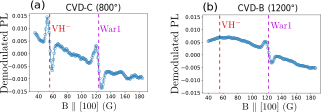
\includegraphics[width=\textwidth]{Figures/VH_CVD_chauffage}
\caption{Demodulated PL on samples CVD-C and CVD-B as a function of a magnetic field along the [100] axis. An additional oscillating magnetic field along the same direction was used to perform the lock-in detection. The VH$^-$ and War1 lines are taken from \ref{CR VH exp}}
\label{chauffage CVD}
\end{figure}

Given that the NV CR spectroscopy was both sensitive and relatively easy to setup, we decided in collaboration with the teams of Alexandre Tallaire at IRCP and Jocelyn Achard at LSPM to study the effect of annealing at high temperature on VH$^-$ and War1 \citep{ngambou2022improving}.

Fig. \ref{chauffage CVD} shows the results of this experiment. This time, a modulation of the magnetic field was used and the PL coming from the photodiode was demodulated through a lock-in amplifier, which explains the derivative shape of the lines. The fact that the background is not perfectly flat still comes from the transverse magnetic field. The same lock-in parameter were used on both plots so that the amplitudes should in theory be comparable.

Fig \ref{chauffage CVD}-a) shows the demodulated PL versus mganetic field amplitude along [100] on sample CVD-C, while \ref{chauffage CVD}-b) shows the same experiment on sample CVD-B. The fabrication and subsequent operations done on this two samples are detailed thoroughly in \citep{ngambou2022improving}, but the main difference between these two sample is that CVD-C was only annealed once after irradiation, for 2 hours at 800$^\circ$C, while CVD-B was annealed for 2 hours at 800$^\circ$C and then for 1 hour at 1000$^\circ$C and 1 hour at 1200$^\circ$C.

We can see that the VH$^-$ line in particular completely disappear on sample CVD-B, which we attribute to the additional annealing. This measurement also corroborate modifications in the infrared absorption spectrum, and an increase of the NV coherence time, associated with the annealing at higher temperature \citep{ngambou2022improving}.

The War1 line on the other hand is still present after the high temperature annealings, albeit slightly smaller. This information can give us some insights on the chemistry of the War1 defect. %Et en vrai je crois que c'était deja vu dans la thèse de Cruddace

\subsection{Modification on HPHT samples}

\begin{figure}[h]
\centering
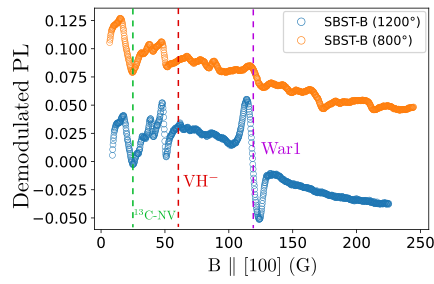
\includegraphics[width=.7\textwidth]{Figures/VH_HPHT_chauffage}
\caption{Demodulated PL on samples SBST-C and SBST-B as a function of a magnetic field along the [100] axis. The plot of SBST-C is offset for clarity}
\label{chauffage HPHT}
\end{figure}

An unexpected side-study was done on HPHT samples. Indeed, the CVD samples used previously are grown by homoepithaxy on top of a diamond substrate. In this case, the substrate was a type 1B HPHT diamond, which was irradiated and annealed along the CVD layer. We Will name SBST-C and SBST-B the respective HPHT substrate of CVD-C and CVD-B.

Fig. \ref{chauffage HPHT} shows demodulated PL scans with B $\parallel$ [100] on both samples. They both show a line at $B \approx 20\ \rm G$ corresponding to the $^{13}$C-NV$^-$ line, and none of them show a line at $B = 56\ \rm G$ corresponding to the VH$^-$ line. There is however a stark difference for the War1 line: SBST-C seems to show a weak line, while SBST-B shows a very clear line, with an amplitude more than 5 times greater than SBST-C. 

We can also see that many weak lines on SBST-B seems to have disappeared in SBST-C, while an unidentified line at $B = 48\ \rm G$ seems to have grown similarly to the War1 line.

We first suspected that some of the War1 defects had been migrating from the CVD layer to the HPHT substrate with the high-temperature annealing, but not only is it very unlikely with the annealing time (1 hour) and substrate thickness (several mm), We also could not find a dependence on the War1 concentration with the depth in the substrate, whereas a diffusion would have given a higher concentration near the CVD layer. The War1 defects seem to have been created by the annealing.

These results suggest that, while some defects are removed by the high temperature annealing, such as the VH$^-$ and several unidentified defects in the HPHT substrate, some seem to be created by the annealing process, such as the War1 or the one associated with the line at $B = 48\ \rm G$ in the HPHT substrate.

\section{Conclusion and perspectives}

To conclude this chapter, we have seen how NV centers can be used to detect dark spins via cross-relaxations. This detection can be way more sensitive than the usual EPR spectroscopy, and considerably cheaper to set up. It is however not as versatile and should be seen as a complimentary tool for diamonds with dense NV ensemble. 

We have also seen the importance of the magnetic field direction, and the underused aspect of the [100] magnetic field scan, much less noisy than the [111] scans for weak magnetic field.

Finally we have seen an application of the CR to detect optically two dark spins in CVD diamond, and to find out the response of these defects to high temperature annealing.

There still remains a lot of open questions and there are several experiments that could be build upon these results. I will list some of them here.

\subsection{Unidentified CR lines}

There are still a large number of lines in CR spectra that have not been identified. While not every line necessarily correspond to a new defect - for example \citep{wunderlich2021magnetic} recently found lines corresponding to co-resonance between the $\ket{0} \to \ket{-1}$ transition of an NV center and the $\ket{-1} \to \ket{+1}$ of another NV center - the more likely hypothesis for each of these unidentified lines is still the presence of a new defect.

Such unidentified lines can be seen in Fig. \ref{chauffage CVD} and \ref{chauffage HPHT}. In particular we can see a line at 160 G in Fig. \ref{chauffage CVD}-a) and a line at 48 G in Fig. \ref{chauffage HPHT} that detach clearly from the background. 

Further studies would be needed to find how common these lines are, and what could be there sources.

\subsection{Measuring the spin dynamics of VH$^-$}

We found that NV-VH$^-$ CR in CVD could produce a change in PL of $\sim 0.2 \%$. This kind of values are not too far from ODMR contrast with NV ensembles, which means that it would be reasonable to probe the dynamics ($T_1$, $T_2$) of the VH$^-$ spin. The main issue comes from the fact that in order to measure the VH$^-$ spin states, it needs to be resonant with the NV center. Therefore, resonant microwave pulses with VH$^-$ will also be resonant with the NV centers, which will create an unwanted optical signal.

There are two solution to circumvent this problem: the first is to use a fast switching magnetic field in order to bring the VH$^-$ and NV centers in resonance when you want to polarize or readout the VH$^-$ state, and out of resonance when you want to coherently manipulate the VH$^-$. This means that the magnetic field needs to be switched faster than the spin dynamics you want to probe. This might be doable for the population dynamics $T_1$ but this is probably too slow to probe the $T_2$ time.

The other solution consists in using the spin-1 nature of VH$^-$: when a NV$^-$-VH$^-$ CR occurs, only one of the transitions of VH$^-$ and NV$^-$ is brought to resonance. The other one ($\ket{0} \to \ket{-1}$ for the VH$^-$) is out of resonance. The idea would therefore be to keep the NV $\ket{0} \to \ket{-1}$ transition and VH $\ket{0} \to \ket{+1}$ transition resonant, and to coherently manipulate the VH $\ket{0} \to \ket{-1}$ transition. While the polarization on this transition, and the back-action it would produce on the NV centers, is not as strong as if you were manipulating the $\ket{0} \to \ket{+1}$ transition, it should still produce a measurable signal.

\subsection{Isolating a single VH$^-$}

We estimated the concentration of VH$^-$ in CVD-pink to be $\sim 60\ \rm ppb$. This concentration is too high by about two orders of magnitude to isolate a single emitter with a diffraction-limited microscope. We know however that we can reduce the VH$^-$ concentration arbitrarily by applying high temperature annealing. We could therefore reduce the VH$^-$ concentration to be in the $0.1 \sim 1\ \rm ppb$ range and optically isolate a single VH$^-$ center by scanning a confocal microscope with a fixed $B_{[100]}=56\ \rm G$ while monitoring the NV PL or $T_1$. It is however unclear to me whether this detection scheme would be sensitive enough to detect single dark spins.

\printbibliography
\end{document}